\documentclass[tikz,border=10pt]{standalone}
\usepackage{amssymb} % for \subset
\usetikzlibrary{arrows.meta, positioning, calc, shapes.geometric}

\begin{document}

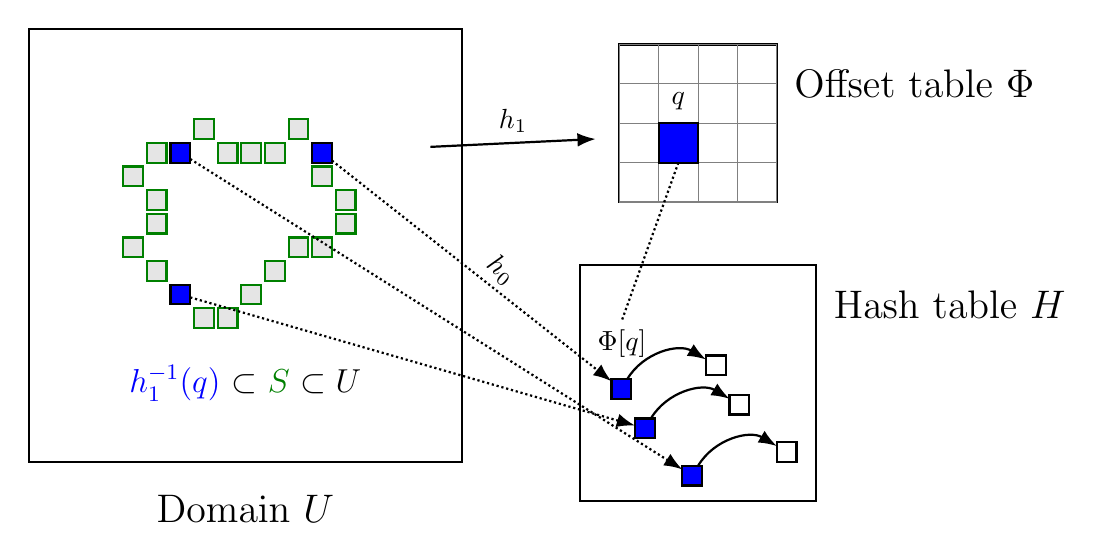
\begin{tikzpicture}[
    >=Latex, % Modern arrow tip
    node distance=1cm,
    % Style definitions
    domain box/.style={draw, thick, rectangle, minimum width=5cm, minimum height=5cm, anchor=south west},
    offset box/.style={draw, thick, rectangle, minimum width=2cm, minimum height=2cm, anchor=south west},
    hash box/.style={draw, thick, rectangle, minimum width=3cm, minimum height=3cm, anchor=south west},
    % Grid cells
    pixel/.style={minimum size=0.25cm, inner sep=0pt, outer sep=0pt, anchor=south west},
    green pixel/.style={pixel, draw=green!50!black, thick, fill=gray!20},
    blue pixel/.style={pixel, draw=black, thick, fill=blue},
    empty pixel/.style={pixel, draw=black, thick, fill=white},
    % Text styles
    label text/.style={font=\Large\rmfamily},
    math text/.style={font=\large}
]

% ==========================================
% 1. DOMAIN U (Left Box)
% ==========================================

% Main Box
\draw[thick] (0,0) rectangle (5.5, 5.5);
\node[label text] at (2.75, -0.6) {Domain $U$};

% Coordinates for the pixel shape
% We use absolute coords relative to (0,0) for simplicity in drawing the "snake"
\def\gx{0.3} % Grid unit size

% -- The Loop Shape (Manually placed to match visual) --

% Top Row
\node[green pixel] at (1.5, 3.8) {}; 
\node[green pixel] at (2.1, 4.1) {}; 
\node[green pixel] at (2.4, 3.8) {}; 
\node[green pixel] at (2.7, 3.8) {}; 
\node[green pixel] at (3.0, 3.8) {}; 
\node[green pixel] at (3.3, 4.1) {}; 


% Left side descending
\node[green pixel] at (1.2, 3.5) {}; 
\node[green pixel] at (1.5, 2.9) {}; 
\node[green pixel] at (1.5, 3.2) {}; 
\node[green pixel] at (1.2, 2.6) {}; 
\node[green pixel] at (1.5, 2.3) {}; 

% Bottom connecting
\node[green pixel] at (2.1, 1.7) {}; 
\node[green pixel] at (2.4, 1.7) {}; 
\node[green pixel] at (2.7, 2.0) {}; 
\node[green pixel] at (3.0, 2.3) {}; 
\node[green pixel] at (3.3, 2.6) {}; 

% Right side connecting
\node[green pixel] at (3.6, 2.6) {}; 
\node[green pixel] at (3.9, 2.9) {}; 
\node[green pixel] at (3.9, 3.2) {}; 
\node[green pixel] at (3.6, 3.5) {}; 

% -- The Three Key Blue Pixels --
% 1. Top Left
\node[blue pixel] (b1) at (1.8, 3.8) {};
% 2. Top Right
\node[blue pixel] (b2) at (3.6, 3.8) {};
% 3. Bottom
\node[blue pixel] (b3) at (1.8, 2.0) {};

% Equation inside Domain
\node at (2.75, 1.0) {\large \textcolor{blue}{$h_1^{-1}(q)$} $\subset$ \textcolor{green!50!black}{$S$} $\subset U$};


% ==========================================
% 2. OFFSET TABLE (Top Right)
% ==========================================

\begin{scope}[shift={(7.5, 3.3)}]
    % Outer Box
    \draw[thick] (0,0) rectangle (2.0, 2.0);
    
    % Internal Grid lines
    \draw[step=0.5cm, gray, thin] (0,0) grid (2.0, 2.0);
    
    % The Blue 'q' Pixel
    \node[blue pixel, minimum size=0.5cm] (q_pixel) at (0.5, 0.5) {};
    \node[above] at (0.75, 1.05) {$q$};
    
    % Label
    \node[label text, anchor=west] at (2.1, 1.5) {Offset table $\Phi$};
\end{scope}


% ==========================================
% 3. HASH TABLE (Bottom Right)
% ==========================================

\begin{scope}[shift={(7.0, -0.5)}]
    % Outer Box
    \draw[thick] (0,0) rectangle (3.0, 3.0);
    
    % Entries (Staggered layout)
    % Entry 1
    \node[blue pixel] (h1_blue) at (0.4, 1.3) {};
    \node[empty pixel] (h1_white) at (1.6, 1.6) {};
    \draw[->, thick, bend left=45] (h1_blue) to (h1_white);
    
    % Entry 2
    \node[blue pixel] (h2_blue) at (0.7, 0.8) {};
    \node[empty pixel] (h2_white) at (1.9, 1.1) {};
    \draw[->, thick, bend left=45] (h2_blue) to (h2_white);
    
    % Entry 3
    \node[blue pixel] (h3_blue) at (1.3, 0.2) {};
    \node[empty pixel] (h3_white) at (2.5, 0.5) {};
    \draw[->, thick, bend left=45] (h3_blue) to (h3_white);

    % Label
    \node[label text, anchor=west] at (3.1, 2.5) {Hash table $H$};
    
    % Label Phi[q]
    \node[anchor=south west] (phi_q_label) at (0.1, 1.7) {$\Phi[q]$};
    % Small arrow from label to first blue block
    %\draw[->] (phi_q_label.south) to [out=270, in=110] (h1_blue.north west);
\end{scope}


% ==========================================
% 4. ARROWS AND CONNECTORS
% ==========================================

% h1 Arrow (Domain -> Offset)
\draw[->, thick] (5.1, 4.0) -- node[above] {$h_1$} (7.2, 4.1);

% Dashed Arrows from Domain to Hash Table (h0)
% We connect the specific blue pixels defined earlier
\draw[densely dotted, thick, ->] (b1) -- (h3_blue);
\draw[densely dotted, thick, ->] (b2) -- (h1_blue);
\draw[densely dotted, thick, ->] (b3) -- (h2_blue);

% Label h0 on the middle line
% We calculate a point along the line for placement
\path (b2) -- node[midway, sloped, above, yshift=2pt] {$h_0$} (h2_blue);

% Dotted line from Offset 'q' to Hash table
\draw[densely dotted, thick] (q_pixel.south) -- (phi_q_label.north);

\end{tikzpicture}

\end{document}